\documentclass[1p]{elsarticle_modified}
%\bibliographystyle{elsarticle-num}

%\usepackage[colorlinks]{hyperref}
%\usepackage{abbrmath_seonhwa} %\Abb, \Ascr, \Acal ,\Abf, \Afrak
\usepackage{amsfonts}
\usepackage{amssymb}
\usepackage{amsmath}
\usepackage{amsthm}
\usepackage{scalefnt}
\usepackage{amsbsy}
\usepackage{kotex}
\usepackage{caption}
\usepackage{subfig}
\usepackage{color}
\usepackage{graphicx}
\usepackage{xcolor} %% white, black, red, green, blue, cyan, magenta, yellow
\usepackage{float}
\usepackage{setspace}
\usepackage{hyperref}

\usepackage{tikz}
\usetikzlibrary{arrows}

\usepackage{multirow}
\usepackage{array} % fixed length table
\usepackage{hhline}

%%%%%%%%%%%%%%%%%%%%%
\makeatletter
\renewcommand*\env@matrix[1][\arraystretch]{%
	\edef\arraystretch{#1}%
	\hskip -\arraycolsep
	\let\@ifnextchar\new@ifnextchar
	\array{*\c@MaxMatrixCols c}}
\makeatother %https://tex.stackexchange.com/questions/14071/how-can-i-increase-the-line-spacing-in-a-matrix
%%%%%%%%%%%%%%%

\usepackage[normalem]{ulem}

\newcommand{\msout}[1]{\ifmmode\text{\sout{\ensuremath{#1}}}\else\sout{#1}\fi}
%SOURCE: \msout is \stkout macro in https://tex.stackexchange.com/questions/20609/strikeout-in-math-mode

\newcommand{\cancel}[1]{
	\ifmmode
	{\color{red}\msout{#1}}
	\else
	{\color{red}\sout{#1}}
	\fi
}

\newcommand{\add}[1]{
	{\color{blue}\uwave{#1}}
}

\newcommand{\replace}[2]{
	\ifmmode
	{\color{red}\msout{#1}}{\color{blue}\uwave{#2}}
	\else
	{\color{red}\sout{#1}}{\color{blue}\uwave{#2}}
	\fi
}

\newcommand{\Sol}{\mathcal{S}} %segment
\newcommand{\D}{D} %diagram
\newcommand{\A}{\mathcal{A}} %arc


%%%%%%%%%%%%%%%%%%%%%%%%%%%%%5 test

\def\sl{\operatorname{\textup{SL}}(2,\Cbb)}
\def\psl{\operatorname{\textup{PSL}}(2,\Cbb)}
\def\quan{\mkern 1mu \triangleright \mkern 1mu}

\theoremstyle{definition}
\newtheorem{thm}{Theorem}[section]
\newtheorem{prop}[thm]{Proposition}
\newtheorem{lem}[thm]{Lemma}
\newtheorem{ques}[thm]{Question}
\newtheorem{cor}[thm]{Corollary}
\newtheorem{defn}[thm]{Definition}
\newtheorem{exam}[thm]{Example}
\newtheorem{rmk}[thm]{Remark}
\newtheorem{alg}[thm]{Algorithm}

\newcommand{\I}{\sqrt{-1}}
\begin{document}

%\begin{frontmatter}
%
%\title{Boundary parabolic representations of knots up to 8 crossings}
%
%%% Group authors per affiliation:
%\author{Yunhi Cho} 
%\address{Department of Mathematics, University of Seoul, Seoul, Korea}
%\ead{yhcho@uos.ac.kr}
%
%
%\author{Seonhwa Kim} %\fnref{s_kim}}
%\address{Center for Geometry and Physics, Institute for Basic Science, Pohang, 37673, Korea}
%\ead{ryeona17@ibs.re.kr}
%
%\author{Hyuk Kim}
%\address{Department of Mathematical Sciences, Seoul National University, Seoul 08826, Korea}
%\ead{hyukkim@snu.ac.kr}
%
%\author{Seokbeom Yoon}
%\address{Department of Mathematical Sciences, Seoul National University, Seoul, 08826,  Korea}
%\ead{sbyoon15@snu.ac.kr}
%
%\begin{abstract}
%We find all boundary parabolic representation of knots up to 8 crossings.
%
%\end{abstract}
%\begin{keyword}
%    \MSC[2010] 57M25 
%\end{keyword}
%
%\end{frontmatter}

%\linenumbers
%\tableofcontents
%
\newcommand\colored[1]{\textcolor{white}{\rule[-0.35ex]{0.8em}{1.4ex}}\kern-0.8em\color{red} #1}%
%\newcommand\colored[1]{\textcolor{white}{ #1}\kern-2.17ex	\textcolor{white}{ #1}\kern-1.81ex	\textcolor{white}{ #1}\kern-2.15ex\color{red}#1	}

{\Large $\underline{12n_{0698}~(K12n_{0698})}$}

\setlength{\tabcolsep}{10pt}
\renewcommand{\arraystretch}{1.6}
\vspace{1cm}\begin{tabular}{m{100pt}>{\centering\arraybackslash}m{274pt}}
\multirow{5}{120pt}{
	\centering
	\includegraphics[width=112pt]{../../../GIT/diagram.site/Diagrams/png/2787_12n_0698.png}\\
\ \ \ A knot diagram\footnotemark}&
\allowdisplaybreaks
\textbf{Linearized knot diagam} \\
\cline{2-2}
 &
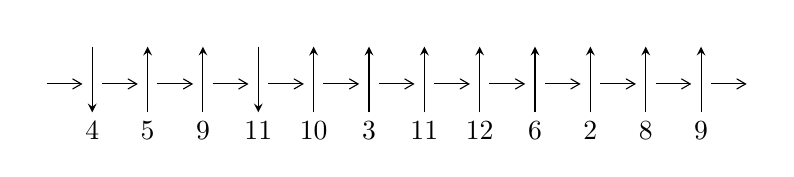
\begin{tikzpicture}[x=20pt, y=17pt]
	% nodes
	\node (C0) at (0, 0) {};
	\node (C1) at (1, 0) {};
	\node (C1U) at (1, +1) {};
	\node (C1D) at (1, -1) {4};

	\node (C2) at (2, 0) {};
	\node (C2U) at (2, +1) {};
	\node (C2D) at (2, -1) {5};

	\node (C3) at (3, 0) {};
	\node (C3U) at (3, +1) {};
	\node (C3D) at (3, -1) {9};

	\node (C4) at (4, 0) {};
	\node (C4U) at (4, +1) {};
	\node (C4D) at (4, -1) {11};

	\node (C5) at (5, 0) {};
	\node (C5U) at (5, +1) {};
	\node (C5D) at (5, -1) {10};

	\node (C6) at (6, 0) {};
	\node (C6U) at (6, +1) {};
	\node (C6D) at (6, -1) {3};

	\node (C7) at (7, 0) {};
	\node (C7U) at (7, +1) {};
	\node (C7D) at (7, -1) {11};

	\node (C8) at (8, 0) {};
	\node (C8U) at (8, +1) {};
	\node (C8D) at (8, -1) {12};

	\node (C9) at (9, 0) {};
	\node (C9U) at (9, +1) {};
	\node (C9D) at (9, -1) {6};

	\node (C10) at (10, 0) {};
	\node (C10U) at (10, +1) {};
	\node (C10D) at (10, -1) {2};

	\node (C11) at (11, 0) {};
	\node (C11U) at (11, +1) {};
	\node (C11D) at (11, -1) {8};

	\node (C12) at (12, 0) {};
	\node (C12U) at (12, +1) {};
	\node (C12D) at (12, -1) {9};
	\node (C13) at (13, 0) {};

	% arrows
	\draw[->,>={angle 60}]
	(C0) edge (C1) (C1) edge (C2) (C2) edge (C3) (C3) edge (C4) (C4) edge (C5) (C5) edge (C6) (C6) edge (C7) (C7) edge (C8) (C8) edge (C9) (C9) edge (C10) (C10) edge (C11) (C11) edge (C12) (C12) edge (C13) ;	\draw[->,>=stealth]
	(C1U) edge (C1D) (C2D) edge (C2U) (C3D) edge (C3U) (C4U) edge (C4D) (C5D) edge (C5U) (C6D) edge (C6U) (C7D) edge (C7U) (C8D) edge (C8U) (C9D) edge (C9U) (C10D) edge (C10U) (C11D) edge (C11U) (C12D) edge (C12U) ;
	\end{tikzpicture} \\
\hhline{~~} \\& 
\textbf{Solving Sequence} \\ \cline{2-2} 
 &
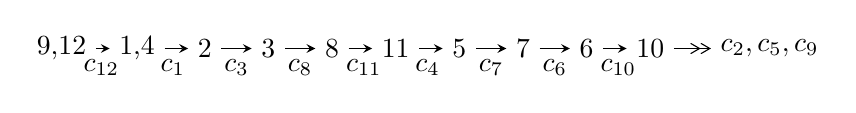
\begin{tikzpicture}[x=23pt, y=7pt]
	% node
	\node (A0) at (-1/8, 0) {9,12};
	\node (A1) at (17/16, 0) {1,4};
	\node (A2) at (17/8, 0) {2};
	\node (A3) at (25/8, 0) {3};
	\node (A4) at (33/8, 0) {8};
	\node (A5) at (41/8, 0) {11};
	\node (A6) at (49/8, 0) {5};
	\node (A7) at (57/8, 0) {7};
	\node (A8) at (65/8, 0) {6};
	\node (A9) at (73/8, 0) {10};
	\node (C1) at (1/2, -1) {$c_{12}$};
	\node (C2) at (13/8, -1) {$c_{1}$};
	\node (C3) at (21/8, -1) {$c_{3}$};
	\node (C4) at (29/8, -1) {$c_{8}$};
	\node (C5) at (37/8, -1) {$c_{11}$};
	\node (C6) at (45/8, -1) {$c_{4}$};
	\node (C7) at (53/8, -1) {$c_{7}$};
	\node (C8) at (61/8, -1) {$c_{6}$};
	\node (C9) at (69/8, -1) {$c_{10}$};
	\node (A10) at (11, 0) {$c_{2},c_{5},c_{9}$};

	% edge
	\draw[->,>=stealth]	
	(A0) edge (A1) (A1) edge (A2) (A2) edge (A3) (A3) edge (A4) (A4) edge (A5) (A5) edge (A6) (A6) edge (A7) (A7) edge (A8) (A8) edge (A9) ;
	\draw[->>,>={angle 60}]	
	(A9) edge (A10);
\end{tikzpicture} \\ 

\end{tabular} \\

\footnotetext{
The image of knot diagram is generated by the software ``\textbf{Draw programme}" developed by Andrew Bartholomew(\url{http://www.layer8.co.uk/maths/draw/index.htm\#Running-draw}), where we modified some parts for our purpose(\url{https://github.com/CATsTAILs/LinksPainter}).
}\phantom \\ \newline 
\centering \textbf{Ideals for irreducible components\footnotemark of $X_{\text{par}}$} 
 
\begin{align*}
I^u_{1}&=\langle 
4.82224\times10^{104} u^{71}+2.70914\times10^{103} u^{70}+\cdots+1.50566\times10^{105} b+5.07425\times10^{105},\\
\phantom{I^u_{1}}&\phantom{= \langle  }-3.95098\times10^{106} u^{71}-5.31311\times10^{105} u^{70}+\cdots+1.95736\times10^{106} a-4.15435\times10^{107},\\
\phantom{I^u_{1}}&\phantom{= \langle  }u^{72}- u^{71}+\cdots+53 u-13\rangle \\
I^u_{2}&=\langle 
55 u^{17}-68 u^{16}+\cdots+b+45,\\
\phantom{I^u_{2}}&\phantom{= \langle  }u^{16}-9 u^{14}+32 u^{12}-54 u^{10}+u^9+33 u^8-5 u^7+23 u^6+8 u^5-39 u^4-4 u^3+10 u^2+a+1,\\
\phantom{I^u_{2}}&\phantom{= \langle  }u^{18}-10 u^{16}+41 u^{14}-86 u^{12}+u^{11}+87 u^{10}-6 u^9-10 u^8+13 u^7-62 u^6-12 u^5+49 u^4+4 u^3-10 u^2+1\rangle \\
\\
\end{align*}
\raggedright * 2 irreducible components of $\dim_{\mathbb{C}}=0$, with total 90 representations.\\
\footnotetext{All coefficients of polynomials are rational numbers. But the coefficients are sometimes approximated in decimal forms when there is not enough margin.}
\newpage
\renewcommand{\arraystretch}{1}
\centering \section*{I. $I^u_{1}= \langle 4.82\times10^{104} u^{71}+2.71\times10^{103} u^{70}+\cdots+1.51\times10^{105} b+5.07\times10^{105},\;-3.95\times10^{106} u^{71}-5.31\times10^{105} u^{70}+\cdots+1.96\times10^{106} a-4.15\times10^{107},\;u^{72}- u^{71}+\cdots+53 u-13 \rangle$}
\flushleft \textbf{(i) Arc colorings}\\
\begin{tabular}{m{7pt} m{180pt} m{7pt} m{180pt} }
\flushright $a_{9}=$&$\begin{pmatrix}0\\u\end{pmatrix}$ \\
\flushright $a_{12}=$&$\begin{pmatrix}1\\0\end{pmatrix}$ \\
\flushright $a_{1}=$&$\begin{pmatrix}1\\- u^2\end{pmatrix}$ \\
\flushright $a_{4}=$&$\begin{pmatrix}2.01852 u^{71}+0.271443 u^{70}+\cdots-65.0023 u+21.2242\\-0.320274 u^{71}-0.0179930 u^{70}+\cdots+10.2838 u-3.37011\end{pmatrix}$ \\
\flushright $a_{2}=$&$\begin{pmatrix}1.34277 u^{71}+0.0225101 u^{70}+\cdots-40.7482 u+15.2242\\-1.75378 u^{71}-0.432113 u^{70}+\cdots+60.3842 u-19.0972\end{pmatrix}$ \\
\flushright $a_{3}=$&$\begin{pmatrix}2.01852 u^{71}+0.271443 u^{70}+\cdots-65.0023 u+21.2242\\2.48267 u^{71}+0.427423 u^{70}+\cdots-84.8436 u+26.3994\end{pmatrix}$ \\
\flushright $a_{8}=$&$\begin{pmatrix}- u\\u\end{pmatrix}$ \\
\flushright $a_{11}=$&$\begin{pmatrix}- u^2+1\\u^2\end{pmatrix}$ \\
\flushright $a_{5}=$&$\begin{pmatrix}0.787391 u^{71}+0.0299893 u^{70}+\cdots-16.9800 u+6.61959\\3.76108 u^{71}+0.707611 u^{70}+\cdots-129.385 u+39.9767\end{pmatrix}$ \\
\flushright $a_{7}=$&$\begin{pmatrix}u^3-2 u\\- u^3+u\end{pmatrix}$ \\
\flushright $a_{6}=$&$\begin{pmatrix}-1.22082 u^{71}-0.484053 u^{70}+\cdots+44.6748 u-14.9450\\0.413411 u^{71}+0.0302634 u^{70}+\cdots+1.23588 u+0.424911\end{pmatrix}$ \\
\flushright $a_{10}=$&$\begin{pmatrix}1.22688 u^{71}+0.0699200 u^{70}+\cdots-40.1232 u+12.0753\\-0.214089 u^{71}+0.417178 u^{70}+\cdots-2.55754 u-0.600644\end{pmatrix}$\\&\end{tabular}
\flushleft \textbf{(ii) Obstruction class $= -1$}\\~\\
\flushleft \textbf{(iii) Cusp Shapes $= -1.82373 u^{71}+0.228275 u^{70}+\cdots+35.3694 u-11.5112$}\\~\\
\newpage\renewcommand{\arraystretch}{1}
\flushleft \textbf{(iv) u-Polynomials at the component}\newline \\
\begin{tabular}{m{50pt}|m{274pt}}
Crossings & \hspace{64pt}u-Polynomials at each crossing \\
\hline $$\begin{aligned}c_{1}\end{aligned}$$&$\begin{aligned}
&u^{72}+6 u^{71}+\cdots-38390 u+1825
\end{aligned}$\\
\hline $$\begin{aligned}c_{2}\end{aligned}$$&$\begin{aligned}
&u^{72}+6 u^{71}+\cdots-228 u+3
\end{aligned}$\\
\hline $$\begin{aligned}c_{3}\end{aligned}$$&$\begin{aligned}
&u^{72}- u^{71}+\cdots-34023 u-7187
\end{aligned}$\\
\hline $$\begin{aligned}c_{4}\end{aligned}$$&$\begin{aligned}
&u^{72}-9 u^{70}+\cdots-3368 u+431
\end{aligned}$\\
\hline $$\begin{aligned}c_{5},c_{9}\end{aligned}$$&$\begin{aligned}
&u^{72}-3 u^{71}+\cdots+99 u-9
\end{aligned}$\\
\hline $$\begin{aligned}c_{6}\end{aligned}$$&$\begin{aligned}
&u^{72}-2 u^{71}+\cdots-1062455 u+98953
\end{aligned}$\\
\hline $$\begin{aligned}c_{7},c_{8},c_{11}\\c_{12}\end{aligned}$$&$\begin{aligned}
&u^{72}- u^{71}+\cdots+53 u-13
\end{aligned}$\\
\hline $$\begin{aligned}c_{10}\end{aligned}$$&$\begin{aligned}
&u^{72}-6 u^{71}+\cdots-1644 u+271
\end{aligned}$\\
\hline
\end{tabular}\\~\\
\newpage\renewcommand{\arraystretch}{1}
\flushleft \textbf{(v) Riley Polynomials at the component}\newline \\
\begin{tabular}{m{50pt}|m{274pt}}
Crossings & \hspace{64pt}Riley Polynomials at each crossing \\
\hline $$\begin{aligned}c_{1}\end{aligned}$$&$\begin{aligned}
&y^{72}-62 y^{71}+\cdots-343686400 y+3330625
\end{aligned}$\\
\hline $$\begin{aligned}c_{2}\end{aligned}$$&$\begin{aligned}
&y^{72}+14 y^{71}+\cdots-66864 y+9
\end{aligned}$\\
\hline $$\begin{aligned}c_{3}\end{aligned}$$&$\begin{aligned}
&y^{72}+61 y^{71}+\cdots+1453616311 y+51652969
\end{aligned}$\\
\hline $$\begin{aligned}c_{4}\end{aligned}$$&$\begin{aligned}
&y^{72}-18 y^{71}+\cdots-35272544 y+185761
\end{aligned}$\\
\hline $$\begin{aligned}c_{5},c_{9}\end{aligned}$$&$\begin{aligned}
&y^{72}+53 y^{71}+\cdots-5265 y+81
\end{aligned}$\\
\hline $$\begin{aligned}c_{6}\end{aligned}$$&$\begin{aligned}
&y^{72}+44 y^{71}+\cdots-139414609387 y+9791696209
\end{aligned}$\\
\hline $$\begin{aligned}c_{7},c_{8},c_{11}\\c_{12}\end{aligned}$$&$\begin{aligned}
&y^{72}-59 y^{71}+\cdots+2755 y+169
\end{aligned}$\\
\hline $$\begin{aligned}c_{10}\end{aligned}$$&$\begin{aligned}
&y^{72}+14 y^{71}+\cdots+1440312 y+73441
\end{aligned}$\\
\hline
\end{tabular}\\~\\
\newpage\flushleft \textbf{(vi) Complex Volumes and Cusp Shapes}
$$\begin{array}{c|c|c}  
\text{Solutions to }I^u_{1}& \I (\text{vol} + \sqrt{-1}CS) & \text{Cusp shape}\\
 \hline 
\begin{aligned}
u &= \phantom{-}0.126859 + 0.988884 I \\
a &= \phantom{-}1.61742 - 0.09689 I \\
b &= \phantom{-}0.050276 - 0.299679 I\end{aligned}
 & -5.20735 + 5.44865 I & \phantom{-0.000000 } 0 \\ \hline\begin{aligned}
u &= \phantom{-}0.126859 - 0.988884 I \\
a &= \phantom{-}1.61742 + 0.09689 I \\
b &= \phantom{-}0.050276 + 0.299679 I\end{aligned}
 & -5.20735 - 5.44865 I & \phantom{-0.000000 } 0 \\ \hline\begin{aligned}
u &= -0.127845 + 1.002920 I \\
a &= \phantom{-}1.70641 + 0.18941 I \\
b &= -0.107709 + 0.230288 I\end{aligned}
 & -10.2342 - 11.1489 I & \phantom{-0.000000 } 0 \\ \hline\begin{aligned}
u &= -0.127845 - 1.002920 I \\
a &= \phantom{-}1.70641 - 0.18941 I \\
b &= -0.107709 - 0.230288 I\end{aligned}
 & -10.2342 + 11.1489 I & \phantom{-0.000000 } 0 \\ \hline\begin{aligned}
u &= -0.141541 + 0.954879 I \\
a &= \phantom{-}1.65626 - 0.08213 I \\
b &= \phantom{-}0.051271 + 0.607650 I\end{aligned}
 & -9.10926 + 1.32235 I & \phantom{-0.000000 } 0 \\ \hline\begin{aligned}
u &= -0.141541 - 0.954879 I \\
a &= \phantom{-}1.65626 + 0.08213 I \\
b &= \phantom{-}0.051271 - 0.607650 I\end{aligned}
 & -9.10926 - 1.32235 I & \phantom{-0.000000 } 0 \\ \hline\begin{aligned}
u &= -0.939877 + 0.013317 I \\
a &= -0.291635 - 1.080060 I \\
b &= \phantom{-}1.73084 + 0.47010 I\end{aligned}
 & -3.34758 + 0.14621 I & \phantom{-}5.65895 + 0. I\phantom{ +0.000000I} \\ \hline\begin{aligned}
u &= -0.939877 - 0.013317 I \\
a &= -0.291635 + 1.080060 I \\
b &= \phantom{-}1.73084 - 0.47010 I\end{aligned}
 & -3.34758 - 0.14621 I & \phantom{-}5.65895 + 0. I\phantom{ +0.000000I} \\ \hline\begin{aligned}
u &= \phantom{-}1.076150 + 0.148518 I \\
a &= -1.37015 + 0.85044 I \\
b &= \phantom{-}2.50989 - 0.59662 I\end{aligned}
 & \phantom{-}2.74768 + 2.38827 I & \phantom{-0.000000 } 0 \\ \hline\begin{aligned}
u &= \phantom{-}1.076150 - 0.148518 I \\
a &= -1.37015 - 0.85044 I \\
b &= \phantom{-}2.50989 + 0.59662 I\end{aligned}
 & \phantom{-}2.74768 - 2.38827 I & \phantom{-0.000000 } 0\\
 \hline 
 \end{array}$$\newpage$$\begin{array}{c|c|c}  
\text{Solutions to }I^u_{1}& \I (\text{vol} + \sqrt{-1}CS) & \text{Cusp shape}\\
 \hline 
\begin{aligned}
u &= \phantom{-}0.169948 + 1.080080 I \\
a &= -1.151840 - 0.173137 I \\
b &= \phantom{-}0.320494 - 0.089757 I\end{aligned}
 & -7.75026 + 1.40505 I & \phantom{-0.000000 } 0 \\ \hline\begin{aligned}
u &= \phantom{-}0.169948 - 1.080080 I \\
a &= -1.151840 + 0.173137 I \\
b &= \phantom{-}0.320494 + 0.089757 I\end{aligned}
 & -7.75026 - 1.40505 I & \phantom{-0.000000 } 0 \\ \hline\begin{aligned}
u &= -0.100523 + 0.879151 I \\
a &= -1.53673 + 0.45497 I \\
b &= \phantom{-}0.235088 - 0.021753 I\end{aligned}
 & -4.60409 + 0.28761 I & \phantom{-}6.69444 + 0.38443 I \\ \hline\begin{aligned}
u &= -0.100523 - 0.879151 I \\
a &= -1.53673 - 0.45497 I \\
b &= \phantom{-}0.235088 + 0.021753 I\end{aligned}
 & -4.60409 - 0.28761 I & \phantom{-}6.69444 - 0.38443 I \\ \hline\begin{aligned}
u &= -0.611340 + 0.627257 I \\
a &= -0.066441 + 0.364149 I \\
b &= -0.206420 + 0.446689 I\end{aligned}
 & -3.02185 - 3.31425 I & \phantom{-}3.79268 + 3.31898 I \\ \hline\begin{aligned}
u &= -0.611340 - 0.627257 I \\
a &= -0.066441 - 0.364149 I \\
b &= -0.206420 - 0.446689 I\end{aligned}
 & -3.02185 + 3.31425 I & \phantom{-}3.79268 - 3.31898 I \\ \hline\begin{aligned}
u &= \phantom{-}1.113140 + 0.172789 I \\
a &= -0.521124 - 0.520349 I \\
b &= \phantom{-}0.45809 - 1.47955 I\end{aligned}
 & \phantom{-}0.00408 + 6.29362 I & \phantom{-0.000000 } 0 \\ \hline\begin{aligned}
u &= \phantom{-}1.113140 - 0.172789 I \\
a &= -0.521124 + 0.520349 I \\
b &= \phantom{-}0.45809 + 1.47955 I\end{aligned}
 & \phantom{-}0.00408 - 6.29362 I & \phantom{-0.000000 } 0 \\ \hline\begin{aligned}
u &= \phantom{-}1.156820 + 0.028330 I \\
a &= \phantom{-}0.165309 + 1.262120 I \\
b &= \phantom{-}0.224082 - 0.645135 I\end{aligned}
 & \phantom{-}3.70030 - 0.68226 I & \phantom{-0.000000 } 0 \\ \hline\begin{aligned}
u &= \phantom{-}1.156820 - 0.028330 I \\
a &= \phantom{-}0.165309 - 1.262120 I \\
b &= \phantom{-}0.224082 + 0.645135 I\end{aligned}
 & \phantom{-}3.70030 + 0.68226 I & \phantom{-0.000000 } 0\\
 \hline 
 \end{array}$$\newpage$$\begin{array}{c|c|c}  
\text{Solutions to }I^u_{1}& \I (\text{vol} + \sqrt{-1}CS) & \text{Cusp shape}\\
 \hline 
\begin{aligned}
u &= -1.167160 + 0.206148 I \\
a &= -1.71705 - 0.04041 I \\
b &= \phantom{-}2.93225 - 0.19622 I\end{aligned}
 & \phantom{-}0.36792 - 7.14775 I & \phantom{-0.000000 } 0 \\ \hline\begin{aligned}
u &= -1.167160 - 0.206148 I \\
a &= -1.71705 + 0.04041 I \\
b &= \phantom{-}2.93225 + 0.19622 I\end{aligned}
 & \phantom{-}0.36792 + 7.14775 I & \phantom{-0.000000 } 0 \\ \hline\begin{aligned}
u &= \phantom{-}0.012163 + 0.813810 I \\
a &= -2.26681 - 0.64788 I \\
b &= \phantom{-}0.353647 + 0.193689 I\end{aligned}
 & -8.47599 - 2.01586 I & -1.74932 + 3.46594 I \\ \hline\begin{aligned}
u &= \phantom{-}0.012163 - 0.813810 I \\
a &= -2.26681 + 0.64788 I \\
b &= \phantom{-}0.353647 - 0.193689 I\end{aligned}
 & -8.47599 + 2.01586 I & -1.74932 - 3.46594 I \\ \hline\begin{aligned}
u &= -1.197050 + 0.139381 I \\
a &= -0.025309 + 0.409207 I \\
b &= -0.278101 + 0.921535 I\end{aligned}
 & \phantom{-}4.25039 - 3.42640 I & \phantom{-0.000000 } 0 \\ \hline\begin{aligned}
u &= -1.197050 - 0.139381 I \\
a &= -0.025309 - 0.409207 I \\
b &= -0.278101 - 0.921535 I\end{aligned}
 & \phantom{-}4.25039 + 3.42640 I & \phantom{-0.000000 } 0 \\ \hline\begin{aligned}
u &= -1.22306\phantom{ +0.000000I} \\
a &= \phantom{-}0.911163\phantom{ +0.000000I} \\
b &= -2.59828\phantom{ +0.000000I}\end{aligned}
 & \phantom{-}5.53230\phantom{ +0.000000I} & \phantom{-0.000000 } 0 \\ \hline\begin{aligned}
u &= \phantom{-}1.257050 + 0.016904 I \\
a &= \phantom{-}0.864368 - 0.363359 I \\
b &= -2.47476 + 1.48717 I\end{aligned}
 & \phantom{-}1.45015 - 3.58564 I & \phantom{-0.000000 } 0 \\ \hline\begin{aligned}
u &= \phantom{-}1.257050 - 0.016904 I \\
a &= \phantom{-}0.864368 + 0.363359 I \\
b &= -2.47476 - 1.48717 I\end{aligned}
 & \phantom{-}1.45015 + 3.58564 I & \phantom{-0.000000 } 0 \\ \hline\begin{aligned}
u &= \phantom{-}1.126030 + 0.582449 I \\
a &= -0.511047 - 0.643523 I \\
b &= \phantom{-}1.44670 + 0.79597 I\end{aligned}
 & -4.85158 + 4.39466 I & \phantom{-0.000000 } 0\\
 \hline 
 \end{array}$$\newpage$$\begin{array}{c|c|c}  
\text{Solutions to }I^u_{1}& \I (\text{vol} + \sqrt{-1}CS) & \text{Cusp shape}\\
 \hline 
\begin{aligned}
u &= \phantom{-}1.126030 - 0.582449 I \\
a &= -0.511047 + 0.643523 I \\
b &= \phantom{-}1.44670 - 0.79597 I\end{aligned}
 & -4.85158 - 4.39466 I & \phantom{-0.000000 } 0 \\ \hline\begin{aligned}
u &= -1.209670 + 0.417858 I \\
a &= -0.856738 + 0.734668 I \\
b &= \phantom{-}1.90170 - 1.11652 I\end{aligned}
 & -1.19160 - 4.92957 I & \phantom{-0.000000 } 0 \\ \hline\begin{aligned}
u &= -1.209670 - 0.417858 I \\
a &= -0.856738 - 0.734668 I \\
b &= \phantom{-}1.90170 + 1.11652 I\end{aligned}
 & -1.19160 + 4.92957 I & \phantom{-0.000000 } 0 \\ \hline\begin{aligned}
u &= \phantom{-}1.272340 + 0.155410 I \\
a &= \phantom{-}0.812489 - 0.086231 I \\
b &= -1.47439 - 0.51290 I\end{aligned}
 & \phantom{-}1.46025 + 2.68807 I & \phantom{-0.000000 } 0 \\ \hline\begin{aligned}
u &= \phantom{-}1.272340 - 0.155410 I \\
a &= \phantom{-}0.812489 + 0.086231 I \\
b &= -1.47439 + 0.51290 I\end{aligned}
 & \phantom{-}1.46025 - 2.68807 I & \phantom{-0.000000 } 0 \\ \hline\begin{aligned}
u &= -1.185310 + 0.498510 I \\
a &= \phantom{-}0.82701 - 1.16892 I \\
b &= -0.71053 + 1.83597 I\end{aligned}
 & -5.90329 - 6.47727 I & \phantom{-0.000000 } 0 \\ \hline\begin{aligned}
u &= -1.185310 - 0.498510 I \\
a &= \phantom{-}0.82701 + 1.16892 I \\
b &= -0.71053 - 1.83597 I\end{aligned}
 & -5.90329 + 6.47727 I & \phantom{-0.000000 } 0 \\ \hline\begin{aligned}
u &= -1.306730 + 0.016350 I \\
a &= \phantom{-}0.763989 + 0.862315 I \\
b &= -0.989243 - 0.377234 I\end{aligned}
 & \phantom{-}2.64593 - 3.47147 I & \phantom{-0.000000 } 0 \\ \hline\begin{aligned}
u &= -1.306730 - 0.016350 I \\
a &= \phantom{-}0.763989 - 0.862315 I \\
b &= -0.989243 + 0.377234 I\end{aligned}
 & \phantom{-}2.64593 + 3.47147 I & \phantom{-0.000000 } 0 \\ \hline\begin{aligned}
u &= \phantom{-}1.185180 + 0.555323 I \\
a &= \phantom{-}0.648873 + 0.912240 I \\
b &= -0.71737 - 1.69599 I\end{aligned}
 & -1.96169 - 0.01375 I & \phantom{-0.000000 } 0\\
 \hline 
 \end{array}$$\newpage$$\begin{array}{c|c|c}  
\text{Solutions to }I^u_{1}& \I (\text{vol} + \sqrt{-1}CS) & \text{Cusp shape}\\
 \hline 
\begin{aligned}
u &= \phantom{-}1.185180 - 0.555323 I \\
a &= \phantom{-}0.648873 - 0.912240 I \\
b &= -0.71737 + 1.69599 I\end{aligned}
 & -1.96169 + 0.01375 I & \phantom{-0.000000 } 0 \\ \hline\begin{aligned}
u &= \phantom{-}1.267320 + 0.374432 I \\
a &= -1.10450 - 1.16691 I \\
b &= \phantom{-}2.31610 + 1.70281 I\end{aligned}
 & -4.57901 + 6.29919 I & \phantom{-0.000000 } 0 \\ \hline\begin{aligned}
u &= \phantom{-}1.267320 - 0.374432 I \\
a &= -1.10450 + 1.16691 I \\
b &= \phantom{-}2.31610 - 1.70281 I\end{aligned}
 & -4.57901 - 6.29919 I & \phantom{-0.000000 } 0 \\ \hline\begin{aligned}
u &= -1.294090 + 0.341511 I \\
a &= -0.290838 + 1.234360 I \\
b &= \phantom{-}1.16609 - 2.28504 I\end{aligned}
 & -4.40911 - 2.13637 I & \phantom{-0.000000 } 0 \\ \hline\begin{aligned}
u &= -1.294090 - 0.341511 I \\
a &= -0.290838 - 1.234360 I \\
b &= \phantom{-}1.16609 + 2.28504 I\end{aligned}
 & -4.40911 + 2.13637 I & \phantom{-0.000000 } 0 \\ \hline\begin{aligned}
u &= -1.204420 + 0.584547 I \\
a &= \phantom{-}0.437650 - 1.000750 I \\
b &= -0.55270 + 1.68415 I\end{aligned}
 & -6.94951 + 5.57839 I & \phantom{-0.000000 } 0 \\ \hline\begin{aligned}
u &= -1.204420 - 0.584547 I \\
a &= \phantom{-}0.437650 + 1.000750 I \\
b &= -0.55270 - 1.68415 I\end{aligned}
 & -6.94951 - 5.57839 I & \phantom{-0.000000 } 0 \\ \hline\begin{aligned}
u &= -0.365082 + 0.449645 I \\
a &= \phantom{-}0.724515 - 0.003907 I \\
b &= \phantom{-}0.590117 + 0.122833 I\end{aligned}
 & -3.33344 - 0.58612 I & \phantom{-}4.42329 + 3.18792 I \\ \hline\begin{aligned}
u &= -0.365082 - 0.449645 I \\
a &= \phantom{-}0.724515 + 0.003907 I \\
b &= \phantom{-}0.590117 - 0.122833 I\end{aligned}
 & -3.33344 + 0.58612 I & \phantom{-}4.42329 - 3.18792 I \\ \hline\begin{aligned}
u &= \phantom{-}1.36594 + 0.40578 I \\
a &= -0.422467 - 0.892800 I \\
b &= \phantom{-}1.05490 + 1.55127 I\end{aligned}
 & \phantom{-}0.01877 + 4.33991 I & \phantom{-0.000000 } 0\\
 \hline 
 \end{array}$$\newpage$$\begin{array}{c|c|c}  
\text{Solutions to }I^u_{1}& \I (\text{vol} + \sqrt{-1}CS) & \text{Cusp shape}\\
 \hline 
\begin{aligned}
u &= \phantom{-}1.36594 - 0.40578 I \\
a &= -0.422467 + 0.892800 I \\
b &= \phantom{-}1.05490 - 1.55127 I\end{aligned}
 & \phantom{-}0.01877 - 4.33991 I & \phantom{-0.000000 } 0 \\ \hline\begin{aligned}
u &= -1.38791 + 0.45935 I \\
a &= \phantom{-}0.810663 - 0.808801 I \\
b &= -1.89548 + 1.84655 I\end{aligned}
 & -0.45597 - 10.62370 I & \phantom{-0.000000 } 0 \\ \hline\begin{aligned}
u &= -1.38791 - 0.45935 I \\
a &= \phantom{-}0.810663 + 0.808801 I \\
b &= -1.89548 - 1.84655 I\end{aligned}
 & -0.45597 + 10.62370 I & \phantom{-0.000000 } 0 \\ \hline\begin{aligned}
u &= \phantom{-}1.39138 + 0.46126 I \\
a &= \phantom{-}0.849080 + 0.942667 I \\
b &= -2.01018 - 1.90844 I\end{aligned}
 & -5.4651 + 16.3720 I & \phantom{-0.000000 } 0 \\ \hline\begin{aligned}
u &= \phantom{-}1.39138 - 0.46126 I \\
a &= \phantom{-}0.849080 - 0.942667 I \\
b &= -2.01018 + 1.90844 I\end{aligned}
 & -5.4651 - 16.3720 I & \phantom{-0.000000 } 0 \\ \hline\begin{aligned}
u &= \phantom{-}1.41047 + 0.44601 I \\
a &= \phantom{-}0.610953 + 0.683746 I \\
b &= -1.76875 - 1.90527 I\end{aligned}
 & -4.21502 + 3.71603 I & \phantom{-0.000000 } 0 \\ \hline\begin{aligned}
u &= \phantom{-}1.41047 - 0.44601 I \\
a &= \phantom{-}0.610953 - 0.683746 I \\
b &= -1.76875 + 1.90527 I\end{aligned}
 & -4.21502 - 3.71603 I & \phantom{-0.000000 } 0 \\ \hline\begin{aligned}
u &= -1.39405 + 0.52910 I \\
a &= -0.526831 + 0.755276 I \\
b &= \phantom{-}1.12722 - 1.11980 I\end{aligned}
 & -2.92127 - 7.14791 I & \phantom{-0.000000 } 0 \\ \hline\begin{aligned}
u &= -1.39405 - 0.52910 I \\
a &= -0.526831 - 0.755276 I \\
b &= \phantom{-}1.12722 + 1.11980 I\end{aligned}
 & -2.92127 + 7.14791 I & \phantom{-0.000000 } 0 \\ \hline\begin{aligned}
u &= \phantom{-}0.365685 + 0.326725 I \\
a &= \phantom{-}1.41373 - 1.37865 I \\
b &= -0.564131 - 0.229982 I\end{aligned}
 & \phantom{-}0.900933 - 0.329550 I & \phantom{-}6.04745 - 3.44320 I\\
 \hline 
 \end{array}$$\newpage$$\begin{array}{c|c|c}  
\text{Solutions to }I^u_{1}& \I (\text{vol} + \sqrt{-1}CS) & \text{Cusp shape}\\
 \hline 
\begin{aligned}
u &= \phantom{-}0.365685 - 0.326725 I \\
a &= \phantom{-}1.41373 + 1.37865 I \\
b &= -0.564131 + 0.229982 I\end{aligned}
 & \phantom{-}0.900933 + 0.329550 I & \phantom{-}6.04745 + 3.44320 I \\ \hline\begin{aligned}
u &= \phantom{-}0.483251\phantom{ +0.000000I} \\
a &= \phantom{-}0.865400\phantom{ +0.000000I} \\
b &= -0.374226\phantom{ +0.000000I}\end{aligned}
 & \phantom{-}0.738726\phantom{ +0.000000I} & \phantom{-}12.8440\phantom{ +0.000000I} \\ \hline\begin{aligned}
u &= \phantom{-}0.271415 + 0.339694 I \\
a &= \phantom{-}1.14210 - 0.85589 I \\
b &= \phantom{-}0.475871 + 1.205610 I\end{aligned}
 & -2.32274 - 4.16974 I & \phantom{-}2.86926 + 0.82016 I \\ \hline\begin{aligned}
u &= \phantom{-}0.271415 - 0.339694 I \\
a &= \phantom{-}1.14210 + 0.85589 I \\
b &= \phantom{-}0.475871 - 1.205610 I\end{aligned}
 & -2.32274 + 4.16974 I & \phantom{-}2.86926 - 0.82016 I \\ \hline\begin{aligned}
u &= -1.58255 + 0.01145 I \\
a &= \phantom{-}0.252185 - 0.123258 I \\
b &= -1.217410 + 0.437776 I\end{aligned}
 & \phantom{-}7.95850 + 0.06427 I & \phantom{-0.000000 } 0 \\ \hline\begin{aligned}
u &= -1.58255 - 0.01145 I \\
a &= \phantom{-}0.252185 + 0.123258 I \\
b &= -1.217410 - 0.437776 I\end{aligned}
 & \phantom{-}7.95850 - 0.06427 I & \phantom{-0.000000 } 0 \\ \hline\begin{aligned}
u &= -0.110595 + 0.398425 I \\
a &= -0.50400 + 3.42521 I \\
b &= -0.525466 - 0.195616 I\end{aligned}
 & -2.69671 + 4.74873 I & \phantom{-}1.03045 - 3.19857 I \\ \hline\begin{aligned}
u &= -0.110595 - 0.398425 I \\
a &= -0.50400 - 3.42521 I \\
b &= -0.525466 + 0.195616 I\end{aligned}
 & -2.69671 - 4.74873 I & \phantom{-}1.03045 + 3.19857 I \\ \hline\begin{aligned}
u &= \phantom{-}1.58743 + 0.13147 I \\
a &= -0.036866 - 0.330156 I \\
b &= -0.272582 + 0.792813 I\end{aligned}
 & \phantom{-}4.58019 + 6.01061 I & \phantom{-0.000000 } 0 \\ \hline\begin{aligned}
u &= \phantom{-}1.58743 - 0.13147 I \\
a &= -0.036866 + 0.330156 I \\
b &= -0.272582 - 0.792813 I\end{aligned}
 & \phantom{-}4.58019 - 6.01061 I & \phantom{-0.000000 } 0\\
 \hline 
 \end{array}$$\newpage$$\begin{array}{c|c|c}  
\text{Solutions to }I^u_{1}& \I (\text{vol} + \sqrt{-1}CS) & \text{Cusp shape}\\
 \hline 
\begin{aligned}
u &= \phantom{-}0.040336 + 0.308718 I \\
a &= \phantom{-}1.162940 + 0.506483 I \\
b &= \phantom{-}0.306872 - 0.876204 I\end{aligned}
 & \phantom{-}0.69881 + 1.66668 I & \phantom{-}4.53475 - 6.54101 I \\ \hline\begin{aligned}
u &= \phantom{-}0.040336 - 0.308718 I \\
a &= \phantom{-}1.162940 - 0.506483 I \\
b &= \phantom{-}0.306872 + 0.876204 I\end{aligned}
 & \phantom{-}0.69881 - 1.66668 I & \phantom{-}4.53475 + 6.54101 I\\
 \hline 
 \end{array}$$\newpage\newpage\renewcommand{\arraystretch}{1}
\centering \section*{II. $I^u_{2}= \langle 55 u^{17}-68 u^{16}+\cdots+b+45,\;u^{16}-9 u^{14}+\cdots+a+1,\;u^{18}-10 u^{16}+\cdots-10 u^2+1 \rangle$}
\flushleft \textbf{(i) Arc colorings}\\
\begin{tabular}{m{7pt} m{180pt} m{7pt} m{180pt} }
\flushright $a_{9}=$&$\begin{pmatrix}0\\u\end{pmatrix}$ \\
\flushright $a_{12}=$&$\begin{pmatrix}1\\0\end{pmatrix}$ \\
\flushright $a_{1}=$&$\begin{pmatrix}1\\- u^2\end{pmatrix}$ \\
\flushright $a_{4}=$&$\begin{pmatrix}- u^{16}+9 u^{14}+\cdots-10 u^2-1\\-55 u^{17}+68 u^{16}+\cdots+35 u-45\end{pmatrix}$ \\
\flushright $a_{2}=$&$\begin{pmatrix}-59 u^{17}+70 u^{16}+\cdots+44 u-48\\119 u^{17}-144 u^{16}+\cdots-80 u+96\end{pmatrix}$ \\
\flushright $a_{3}=$&$\begin{pmatrix}- u^{16}+9 u^{14}+\cdots-10 u^2-1\\-55 u^{17}+67 u^{16}+\cdots+35 u-44\end{pmatrix}$ \\
\flushright $a_{8}=$&$\begin{pmatrix}- u\\u\end{pmatrix}$ \\
\flushright $a_{11}=$&$\begin{pmatrix}- u^2+1\\u^2\end{pmatrix}$ \\
\flushright $a_{5}=$&$\begin{pmatrix}13 u^{17}-17 u^{16}+\cdots-8 u+9\\-96 u^{17}+116 u^{16}+\cdots+63 u-77\end{pmatrix}$ \\
\flushright $a_{7}=$&$\begin{pmatrix}u^3-2 u\\- u^3+u\end{pmatrix}$ \\
\flushright $a_{6}=$&$\begin{pmatrix}-37 u^{17}+44 u^{16}+\cdots+23 u-32\\54 u^{17}-67 u^{16}+\cdots-32 u+44\end{pmatrix}$ \\
\flushright $a_{10}=$&$\begin{pmatrix}-16 u^{17}+21 u^{16}+\cdots+4 u-10\\-19 u^{17}+22 u^{16}+\cdots+15 u-16\end{pmatrix}$\\&\end{tabular}
\flushleft \textbf{(ii) Obstruction class $= 1$}\\~\\
\flushleft \textbf{(iii) Cusp Shapes $= -230 u^{17}+282 u^{16}+1952 u^{15}-2397 u^{14}-6471 u^{13}+7965 u^{12}+9941 u^{11}-12521 u^{10}-4527 u^9+7084 u^8-6484 u^7+4905 u^6+8225 u^5-7445 u^4-2069 u^3+1737 u^2+144 u-174$}\\~\\
\newpage\renewcommand{\arraystretch}{1}
\flushleft \textbf{(iv) u-Polynomials at the component}\newline \\
\begin{tabular}{m{50pt}|m{274pt}}
Crossings & \hspace{64pt}u-Polynomials at each crossing \\
\hline $$\begin{aligned}c_{1}\end{aligned}$$&$\begin{aligned}
&u^{18}-11 u^{17}+\cdots-39 u+5
\end{aligned}$\\
\hline $$\begin{aligned}c_{2}\end{aligned}$$&$\begin{aligned}
&u^{18}+7 u^{17}+\cdots+3 u+1
\end{aligned}$\\
\hline $$\begin{aligned}c_{3}\end{aligned}$$&$\begin{aligned}
&u^{18}+2 u^{16}+\cdots-6 u^2+1
\end{aligned}$\\
\hline $$\begin{aligned}c_{4}\end{aligned}$$&$\begin{aligned}
&u^{18}- u^{17}+\cdots- u+1
\end{aligned}$\\
\hline $$\begin{aligned}c_{5}\end{aligned}$$&$\begin{aligned}
&u^{18}-2 u^{17}+\cdots-8 u+5
\end{aligned}$\\
\hline $$\begin{aligned}c_{6}\end{aligned}$$&$\begin{aligned}
&u^{18}+3 u^{17}+\cdots-6 u+1
\end{aligned}$\\
\hline $$\begin{aligned}c_{7},c_{8}\end{aligned}$$&$\begin{aligned}
&u^{18}-10 u^{16}+\cdots-10 u^2+1
\end{aligned}$\\
\hline $$\begin{aligned}c_{9}\end{aligned}$$&$\begin{aligned}
&u^{18}+2 u^{17}+\cdots+8 u+5
\end{aligned}$\\
\hline $$\begin{aligned}c_{10}\end{aligned}$$&$\begin{aligned}
&u^{18}- u^{17}+\cdots- u+1
\end{aligned}$\\
\hline $$\begin{aligned}c_{11},c_{12}\end{aligned}$$&$\begin{aligned}
&u^{18}-10 u^{16}+\cdots-10 u^2+1
\end{aligned}$\\
\hline
\end{tabular}\\~\\
\newpage\renewcommand{\arraystretch}{1}
\flushleft \textbf{(v) Riley Polynomials at the component}\newline \\
\begin{tabular}{m{50pt}|m{274pt}}
Crossings & \hspace{64pt}Riley Polynomials at each crossing \\
\hline $$\begin{aligned}c_{1}\end{aligned}$$&$\begin{aligned}
&y^{18}-3 y^{17}+\cdots+169 y+25
\end{aligned}$\\
\hline $$\begin{aligned}c_{2}\end{aligned}$$&$\begin{aligned}
&y^{18}+y^{17}+\cdots-7 y+1
\end{aligned}$\\
\hline $$\begin{aligned}c_{3}\end{aligned}$$&$\begin{aligned}
&y^{18}+4 y^{17}+\cdots-12 y+1
\end{aligned}$\\
\hline $$\begin{aligned}c_{4}\end{aligned}$$&$\begin{aligned}
&y^{18}+y^{17}+\cdots-3 y+1
\end{aligned}$\\
\hline $$\begin{aligned}c_{5},c_{9}\end{aligned}$$&$\begin{aligned}
&y^{18}+12 y^{17}+\cdots+116 y+25
\end{aligned}$\\
\hline $$\begin{aligned}c_{6}\end{aligned}$$&$\begin{aligned}
&y^{18}+11 y^{17}+\cdots-10 y+1
\end{aligned}$\\
\hline $$\begin{aligned}c_{7},c_{8},c_{11}\\c_{12}\end{aligned}$$&$\begin{aligned}
&y^{18}-20 y^{17}+\cdots-20 y+1
\end{aligned}$\\
\hline $$\begin{aligned}c_{10}\end{aligned}$$&$\begin{aligned}
&y^{18}-3 y^{17}+\cdots+y+1
\end{aligned}$\\
\hline
\end{tabular}\\~\\
\newpage\flushleft \textbf{(vi) Complex Volumes and Cusp Shapes}
$$\begin{array}{c|c|c}  
\text{Solutions to }I^u_{2}& \I (\text{vol} + \sqrt{-1}CS) & \text{Cusp shape}\\
 \hline 
\begin{aligned}
u &= \phantom{-}0.034780 + 0.909417 I \\
a &= -1.54704 - 0.01895 I \\
b &= \phantom{-}0.338766 - 0.248147 I\end{aligned}
 & -6.97448 + 1.13968 I & \phantom{-}4.89374 - 0.18325 I \\ \hline\begin{aligned}
u &= \phantom{-}0.034780 - 0.909417 I \\
a &= -1.54704 + 0.01895 I \\
b &= \phantom{-}0.338766 + 0.248147 I\end{aligned}
 & -6.97448 - 1.13968 I & \phantom{-}4.89374 + 0.18325 I \\ \hline\begin{aligned}
u &= \phantom{-}1.207980 + 0.098270 I \\
a &= \phantom{-}0.739289 - 0.918515 I \\
b &= -1.354920 + 0.330046 I\end{aligned}
 & \phantom{-}4.03681 + 2.12143 I & \phantom{-}15.7293 - 1.9822 I \\ \hline\begin{aligned}
u &= \phantom{-}1.207980 - 0.098270 I \\
a &= \phantom{-}0.739289 + 0.918515 I \\
b &= -1.354920 - 0.330046 I\end{aligned}
 & \phantom{-}4.03681 - 2.12143 I & \phantom{-}15.7293 + 1.9822 I \\ \hline\begin{aligned}
u &= -1.221290 + 0.000878 I \\
a &= \phantom{-}1.034340 + 0.008877 I \\
b &= -1.83950 - 1.59017 I\end{aligned}
 & \phantom{-}1.08464 + 4.68616 I & \phantom{-}9.18075 - 6.62870 I \\ \hline\begin{aligned}
u &= -1.221290 - 0.000878 I \\
a &= \phantom{-}1.034340 - 0.008877 I \\
b &= -1.83950 + 1.59017 I\end{aligned}
 & \phantom{-}1.08464 - 4.68616 I & \phantom{-}9.18075 + 6.62870 I \\ \hline\begin{aligned}
u &= -1.242500 + 0.470628 I \\
a &= -0.780988 + 0.794704 I \\
b &= \phantom{-}1.46588 - 0.99279 I\end{aligned}
 & -3.02478 - 6.13837 I & \phantom{-}6.43166 + 4.31912 I \\ \hline\begin{aligned}
u &= -1.242500 - 0.470628 I \\
a &= -0.780988 - 0.794704 I \\
b &= \phantom{-}1.46588 + 0.99279 I\end{aligned}
 & -3.02478 + 6.13837 I & \phantom{-}6.43166 - 4.31912 I \\ \hline\begin{aligned}
u &= \phantom{-}1.297070 + 0.392739 I \\
a &= -0.598955 - 0.773625 I \\
b &= \phantom{-}1.81748 + 1.61626 I\end{aligned}
 & -3.07920 + 3.40899 I & \phantom{-}8.53631 - 2.87922 I \\ \hline\begin{aligned}
u &= \phantom{-}1.297070 - 0.392739 I \\
a &= -0.598955 + 0.773625 I \\
b &= \phantom{-}1.81748 - 1.61626 I\end{aligned}
 & -3.07920 - 3.40899 I & \phantom{-}8.53631 + 2.87922 I\\
 \hline 
 \end{array}$$\newpage$$\begin{array}{c|c|c}  
\text{Solutions to }I^u_{2}& \I (\text{vol} + \sqrt{-1}CS) & \text{Cusp shape}\\
 \hline 
\begin{aligned}
u &= \phantom{-}1.53345 + 0.10123 I \\
a &= -0.292336 - 0.163807 I \\
b &= \phantom{-}0.743032 - 0.190463 I\end{aligned}
 & \phantom{-}5.16035 + 6.11216 I & \phantom{-}16.2770 - 5.8147 I \\ \hline\begin{aligned}
u &= \phantom{-}1.53345 - 0.10123 I \\
a &= -0.292336 + 0.163807 I \\
b &= \phantom{-}0.743032 + 0.190463 I\end{aligned}
 & \phantom{-}5.16035 - 6.11216 I & \phantom{-}16.2770 + 5.8147 I \\ \hline\begin{aligned}
u &= -1.56582 + 0.04096 I \\
a &= -0.315755 + 0.060524 I \\
b &= \phantom{-}1.35534 - 0.49741 I\end{aligned}
 & \phantom{-}8.11860 + 0.22024 I & \phantom{-}22.9414 - 14.5563 I \\ \hline\begin{aligned}
u &= -1.56582 - 0.04096 I \\
a &= -0.315755 - 0.060524 I \\
b &= \phantom{-}1.35534 + 0.49741 I\end{aligned}
 & \phantom{-}8.11860 - 0.22024 I & \phantom{-}22.9414 + 14.5563 I \\ \hline\begin{aligned}
u &= -0.403896 + 0.125852 I \\
a &= -2.15630 + 0.13786 I \\
b &= \phantom{-}0.415201 + 0.902527 I\end{aligned}
 & -1.63695 - 4.97346 I & \phantom{-}9.65134 + 6.36185 I \\ \hline\begin{aligned}
u &= -0.403896 - 0.125852 I \\
a &= -2.15630 - 0.13786 I \\
b &= \phantom{-}0.415201 - 0.902527 I\end{aligned}
 & -1.63695 + 4.97346 I & \phantom{-}9.65134 - 6.36185 I \\ \hline\begin{aligned}
u &= \phantom{-}0.360211 + 0.184792 I \\
a &= -2.08226 - 0.15931 I \\
b &= \phantom{-}0.558708 + 0.874453 I\end{aligned}
 & \phantom{-}1.24981 - 1.03640 I & \phantom{-}10.85847 + 2.38119 I \\ \hline\begin{aligned}
u &= \phantom{-}0.360211 - 0.184792 I \\
a &= -2.08226 + 0.15931 I \\
b &= \phantom{-}0.558708 - 0.874453 I\end{aligned}
 & \phantom{-}1.24981 + 1.03640 I & \phantom{-}10.85847 - 2.38119 I\\
 \hline 
 \end{array}$$\newpage
\newpage\renewcommand{\arraystretch}{1}
\centering \section*{ III. u-Polynomials}
\begin{tabular}{m{50pt}|m{274pt}}
Crossings & \hspace{64pt}u-Polynomials at each crossing \\
\hline $$\begin{aligned}c_{1}\end{aligned}$$&$\begin{aligned}
&(u^{18}-11 u^{17}+\cdots-39 u+5)(u^{72}+6 u^{71}+\cdots-38390 u+1825)
\end{aligned}$\\
\hline $$\begin{aligned}c_{2}\end{aligned}$$&$\begin{aligned}
&(u^{18}+7 u^{17}+\cdots+3 u+1)(u^{72}+6 u^{71}+\cdots-228 u+3)
\end{aligned}$\\
\hline $$\begin{aligned}c_{3}\end{aligned}$$&$\begin{aligned}
&(u^{18}+2 u^{16}+\cdots-6 u^2+1)(u^{72}- u^{71}+\cdots-34023 u-7187)
\end{aligned}$\\
\hline $$\begin{aligned}c_{4}\end{aligned}$$&$\begin{aligned}
&(u^{18}- u^{17}+\cdots- u+1)(u^{72}-9 u^{70}+\cdots-3368 u+431)
\end{aligned}$\\
\hline $$\begin{aligned}c_{5}\end{aligned}$$&$\begin{aligned}
&(u^{18}-2 u^{17}+\cdots-8 u+5)(u^{72}-3 u^{71}+\cdots+99 u-9)
\end{aligned}$\\
\hline $$\begin{aligned}c_{6}\end{aligned}$$&$\begin{aligned}
&(u^{18}+3 u^{17}+\cdots-6 u+1)(u^{72}-2 u^{71}+\cdots-1062455 u+98953)
\end{aligned}$\\
\hline $$\begin{aligned}c_{7},c_{8}\end{aligned}$$&$\begin{aligned}
&(u^{18}-10 u^{16}+\cdots-10 u^2+1)(u^{72}- u^{71}+\cdots+53 u-13)
\end{aligned}$\\
\hline $$\begin{aligned}c_{9}\end{aligned}$$&$\begin{aligned}
&(u^{18}+2 u^{17}+\cdots+8 u+5)(u^{72}-3 u^{71}+\cdots+99 u-9)
\end{aligned}$\\
\hline $$\begin{aligned}c_{10}\end{aligned}$$&$\begin{aligned}
&(u^{18}- u^{17}+\cdots- u+1)(u^{72}-6 u^{71}+\cdots-1644 u+271)
\end{aligned}$\\
\hline $$\begin{aligned}c_{11},c_{12}\end{aligned}$$&$\begin{aligned}
&(u^{18}-10 u^{16}+\cdots-10 u^2+1)(u^{72}- u^{71}+\cdots+53 u-13)
\end{aligned}$\\
\hline
\end{tabular}\newpage\renewcommand{\arraystretch}{1}
\centering \section*{ IV. Riley Polynomials}
\begin{tabular}{m{50pt}|m{274pt}}
Crossings & \hspace{64pt}Riley Polynomials at each crossing \\
\hline $$\begin{aligned}c_{1}\end{aligned}$$&$\begin{aligned}
&(y^{18}-3 y^{17}+\cdots+169 y+25)\\
&\cdot(y^{72}-62 y^{71}+\cdots-343686400 y+3330625)
\end{aligned}$\\
\hline $$\begin{aligned}c_{2}\end{aligned}$$&$\begin{aligned}
&(y^{18}+y^{17}+\cdots-7 y+1)(y^{72}+14 y^{71}+\cdots-66864 y+9)
\end{aligned}$\\
\hline $$\begin{aligned}c_{3}\end{aligned}$$&$\begin{aligned}
&(y^{18}+4 y^{17}+\cdots-12 y+1)\\
&\cdot(y^{72}+61 y^{71}+\cdots+1453616311 y+51652969)
\end{aligned}$\\
\hline $$\begin{aligned}c_{4}\end{aligned}$$&$\begin{aligned}
&(y^{18}+y^{17}+\cdots-3 y+1)(y^{72}-18 y^{71}+\cdots-3.52725\times10^{7} y+185761)
\end{aligned}$\\
\hline $$\begin{aligned}c_{5},c_{9}\end{aligned}$$&$\begin{aligned}
&(y^{18}+12 y^{17}+\cdots+116 y+25)(y^{72}+53 y^{71}+\cdots-5265 y+81)
\end{aligned}$\\
\hline $$\begin{aligned}c_{6}\end{aligned}$$&$\begin{aligned}
&(y^{18}+11 y^{17}+\cdots-10 y+1)\\
&\cdot(y^{72}+44 y^{71}+\cdots-139414609387 y+9791696209)
\end{aligned}$\\
\hline $$\begin{aligned}c_{7},c_{8},c_{11}\\c_{12}\end{aligned}$$&$\begin{aligned}
&(y^{18}-20 y^{17}+\cdots-20 y+1)(y^{72}-59 y^{71}+\cdots+2755 y+169)
\end{aligned}$\\
\hline $$\begin{aligned}c_{10}\end{aligned}$$&$\begin{aligned}
&(y^{18}-3 y^{17}+\cdots+y+1)(y^{72}+14 y^{71}+\cdots+1440312 y+73441)
\end{aligned}$\\
\hline
\end{tabular}
\vskip 2pc
\end{document}